\documentclass[10pt]{beamer}

\usetheme[progressbar=frametitle]{metropolis}
\usepackage{appendixnumberbeamer}
\usepackage{graphicx}
\usepackage{booktabs}
\usepackage[scale=2]{ccicons}
\usepackage[space]{xeCJK}
\usepackage{pgfplots}
\usepgfplotslibrary{dateplot}

\usepackage{xspace}
\newcommand{\themename}{\textbf{\textsc{metropolis}}\xspace}

\pagestyle{empty}

\title{KA-Ensemble }
\subtitle{Towards Imbalanced Image Classification Ensembling Over-samling and Under-sampling}
\date{\today}
%\date{}
\author{Hao Ding}
\institute{Ocean Univercity of China}
\titlegraphic{\hfill
\includegraphics[height=1.5cm]{zhenglab-logo.png}}

\begin{document}

\maketitle

\begin{frame}{Table of contents}
  \setbeamertemplate{section in toc}[sections numbered]
  \tableofcontents[hideallsubsections]
\end{frame}

\section{Imbalanced learning}

\begin{frame}[fragile]{Imbalanced learning}

\begin{figure}[!ht]
\centering
  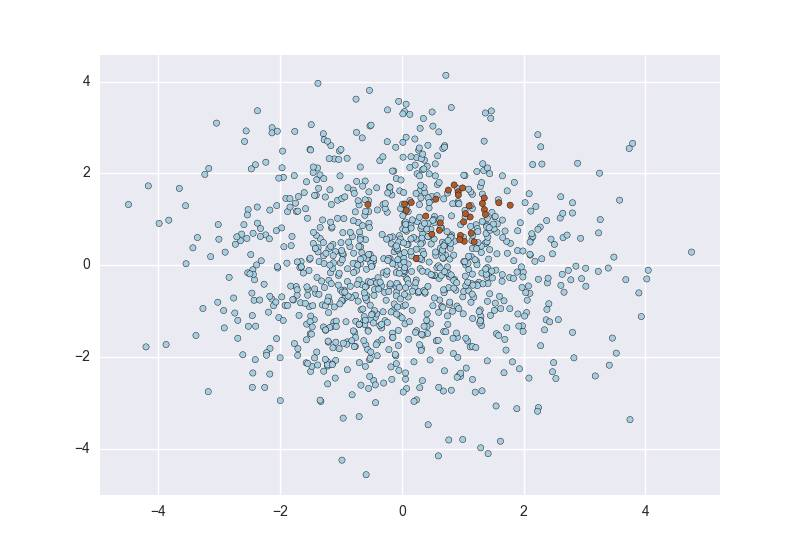
\includegraphics[width=\linewidth]{0}
  \label{fig:a}
%\caption{method}
  %\hspace{0.05in}  
\end{figure}
\end{frame}

\begin{frame}[fragile]{Sampling method}

According to the different sort of samples, sampling methods can be roughly classified into three classes: 
\begin{itemize}
\item over-sampling
\item under-sampling
\item hybrid-sampling
\end{itemize}
  
\end{frame}

%\begin{frame}[fragile]{Sampling method}

%According to the different sort of samples, sampling methods can be roughly classified into three classes: 
%\begin{itemize}
%\item over-sampling
%\item under-sampling
%\item hybrid-sampling
%\end{itemize}
%\alert{Always do k-fold Cross-validation when over sampling}

%\end{frame}

\section{Method}

\begin{frame}{SMOTE}
\begin{figure}[!ht]
\centering
  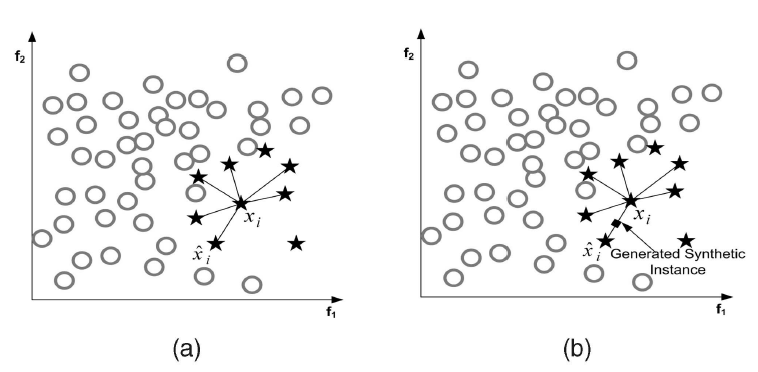
\includegraphics[width=\linewidth]{smote}
 %\label{fig:a}
%\caption{method}
  %\hspace{0.05in}  
\end{figure}
\end{frame}


\begin{frame}{ADASYN}
 \begin{itemize}
  \item Calculate how many minority samples to generate ($N^{+}*SR$).
  \item For each minority sample $x^{+}_{i},i=1,2,...,N^{+}$, find its K-nearest neighbors, $N_{i}^{maj}$ of which from the majority.
  \item $\Gamma_{i}=\frac{\frac{N_{i}^{maj}}{K}}{Z}$, Z is a standardization factor to make sure $\sum \Gamma _{i}=1$
  \item $g_{i}=\Gamma _{i}*N^{+}*SR$
 \end{itemize}
 \end{frame}

\begin{frame}{ADASYN}

\textbf{ Pros:} Adaptively determine the frequency of each minority sample as the primary sample and focus the attention on the boundary regions of the minority class.

 \textbf{ Cons:} The anti-noise performance of the algorithm is poor, which will amplify the range of small-scale noise information to a certain extent, resulting in a decline in classification quality.
\end{frame}

\begin{frame}{Kernal ADASYN}
kernal density estimation:

$\hat{p}(x)=\frac{1}{N+h} \sum_{i\in I_{+1}} \hat{r_i} \frac{1}{(\sqrt{2\pi}h)^n} exp(-\frac{1}{2}\frac{|x-x_i|}{h})$\\
\vspace{2em}
Not only  adaptively shifting the classification decision boundary toward the difficult examples. 

But also construct an adaptive over-sampling distribution to generate synthetic minority class data.
\end{frame}

\begin{frame}{Kernal ADASYN}
\begin{figure}[!ht]
\centering
  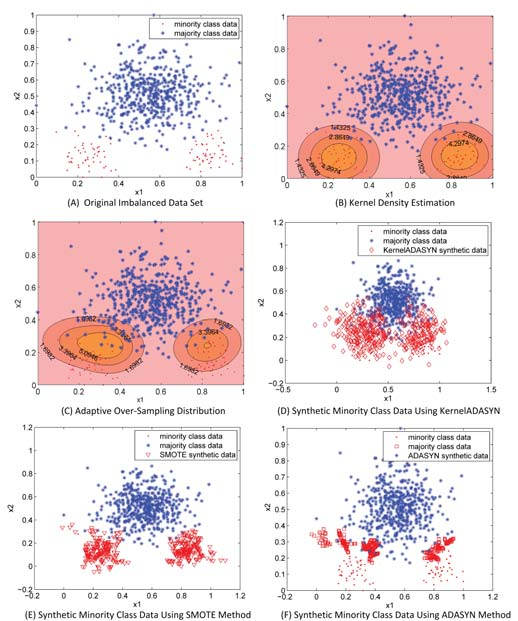
\includegraphics[width=0.6\linewidth]{KADASYN}
\end{figure}
\end{frame}

\begin{frame}{EasyEnsemble}
\begin{figure}[!ht]
\centering
  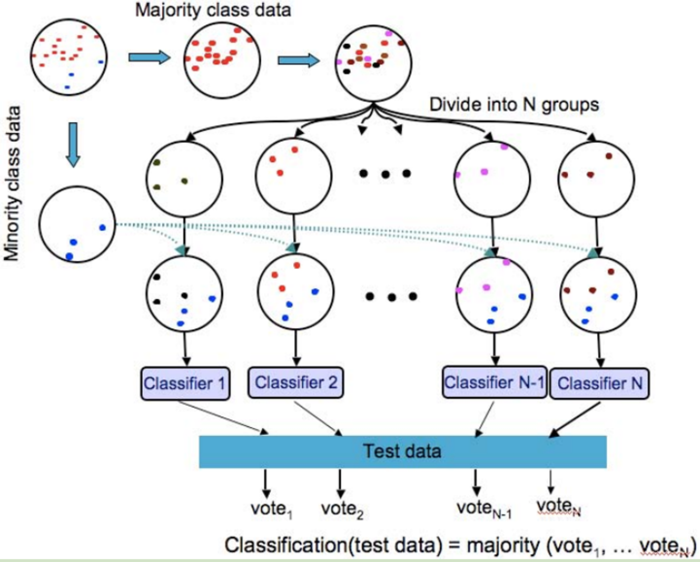
\includegraphics[width=0.8\linewidth]{easy}
 %\label{fig:a}
%\caption{method}
  %\hspace{0.05in}  
\end{figure}
\end{frame}

\begin{frame}{KA-Ensemble}

\begin{figure}[!ht]
\centering
  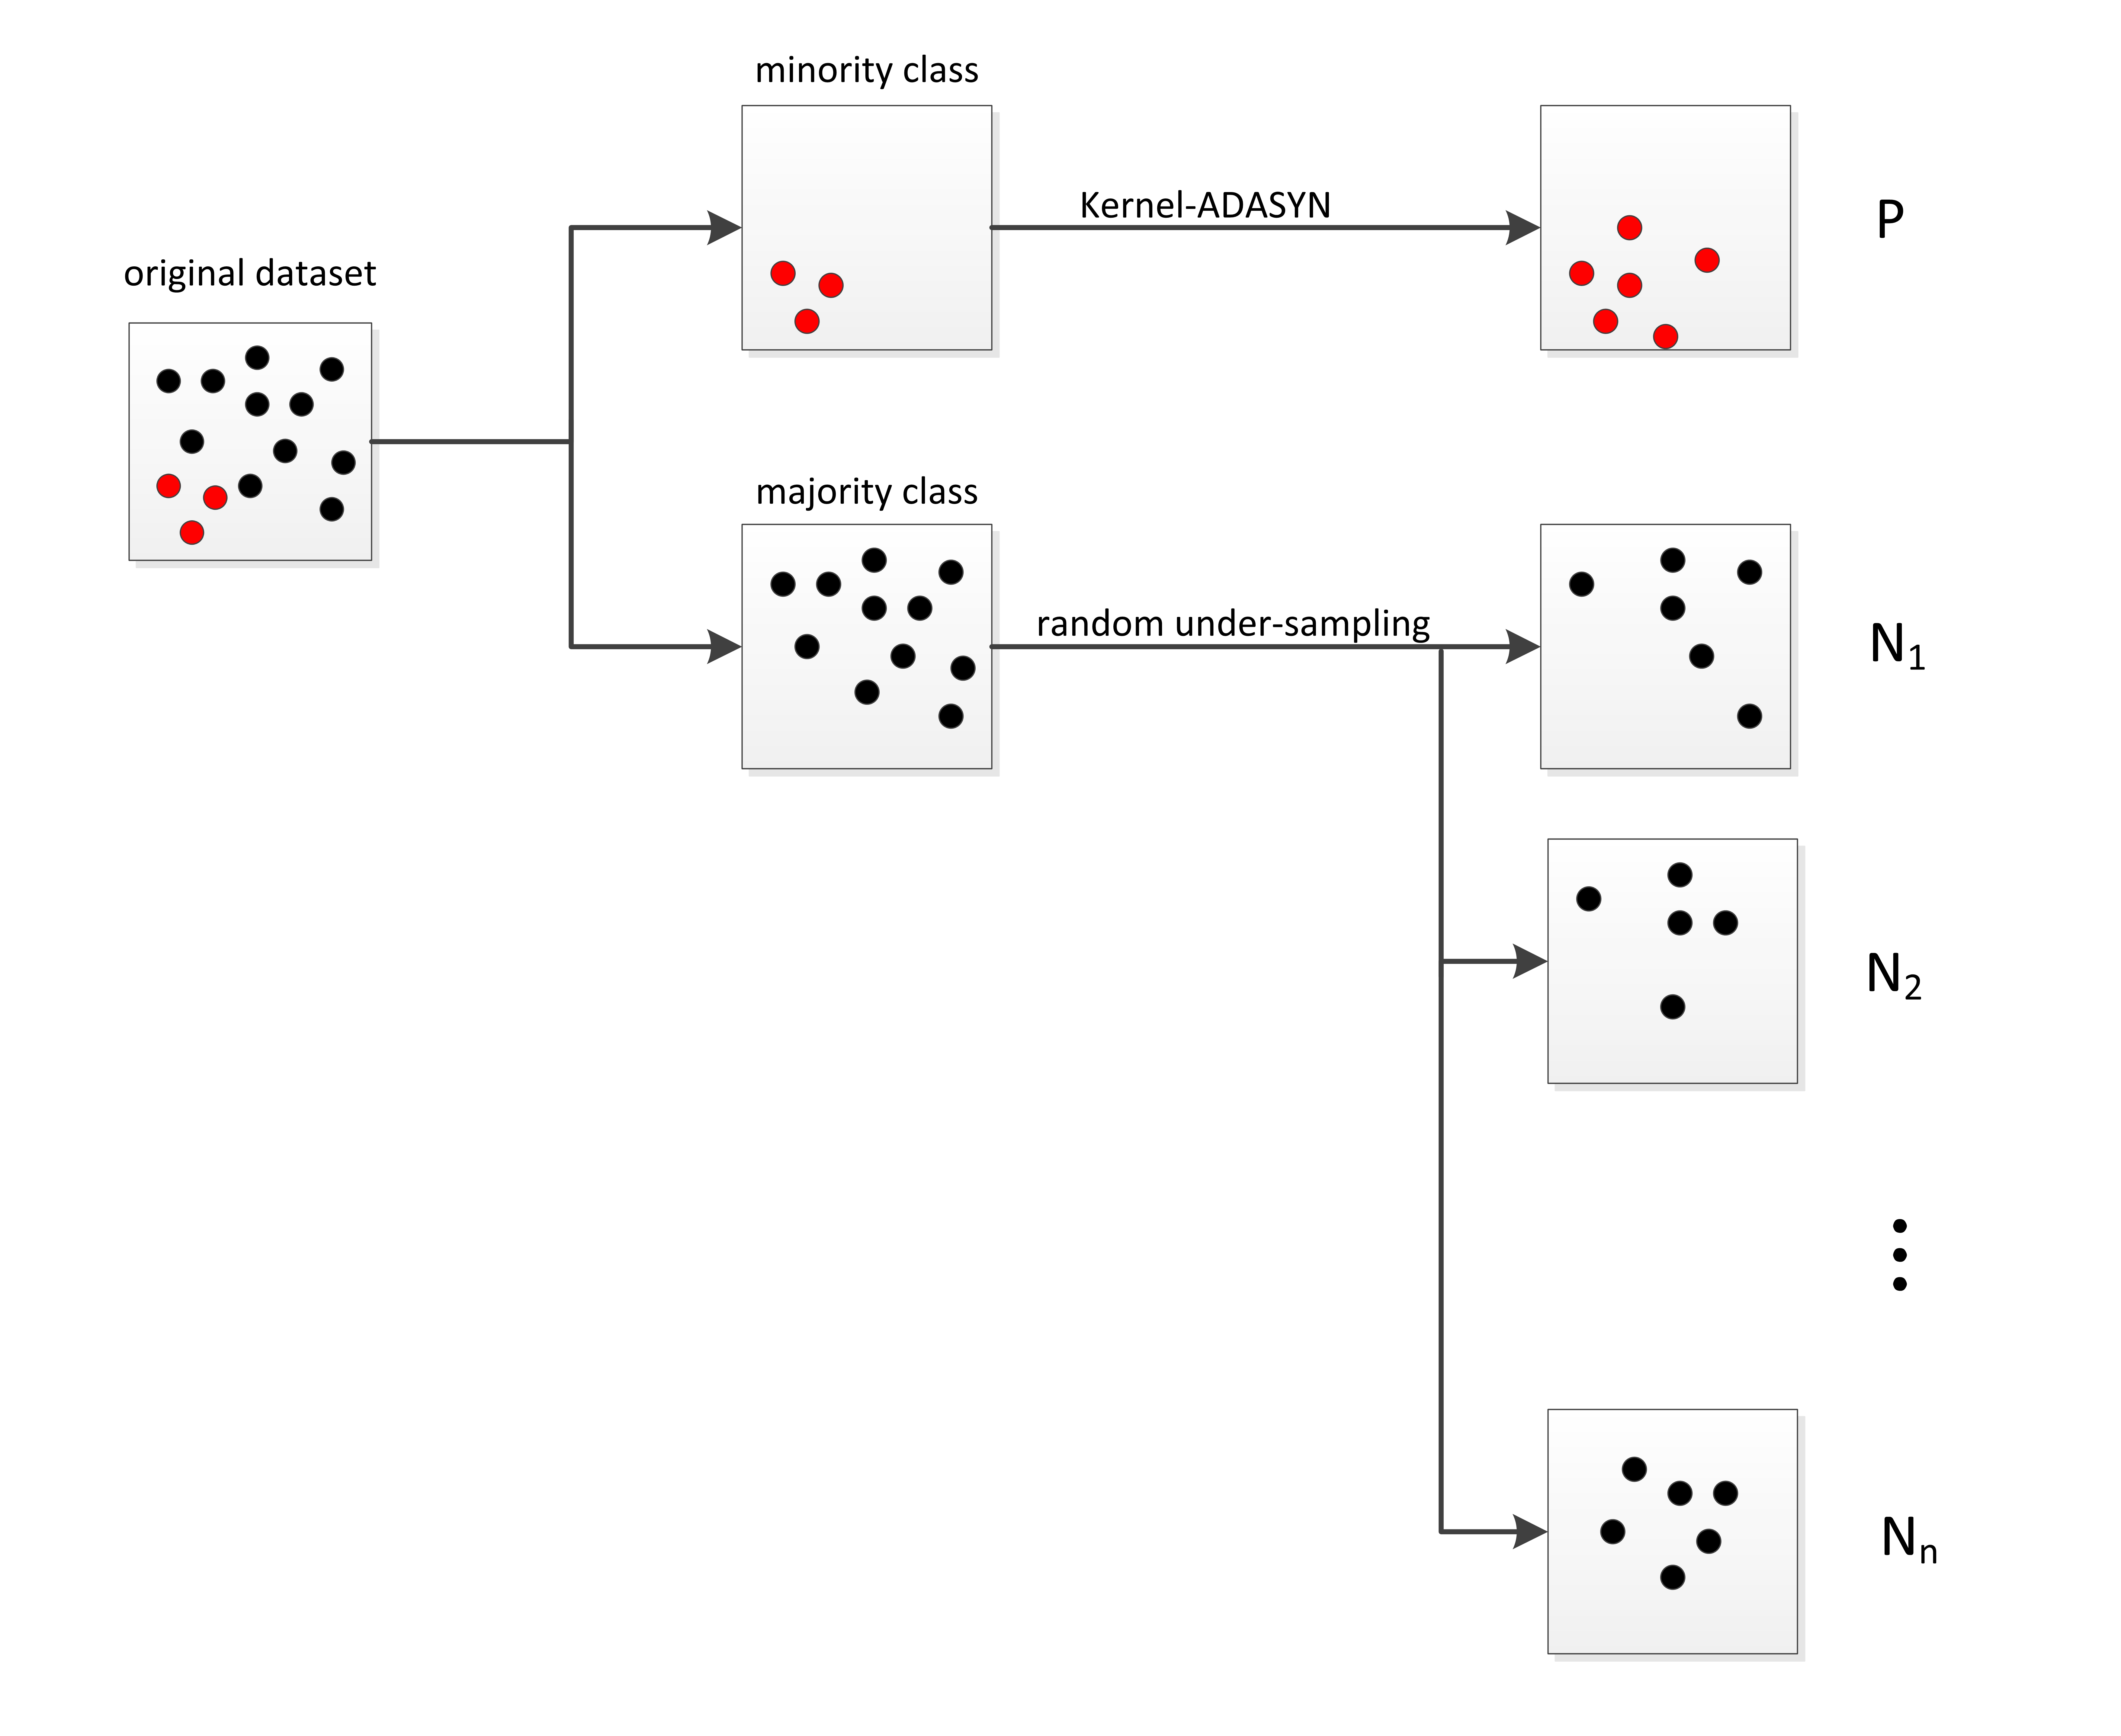
\includegraphics[width=0.55\linewidth]{method}
%  \label{fig:a}
%\caption{method}
  %\hspace{0.05in}  
\end{figure}

\begin{figure}[!ht]
\centering
  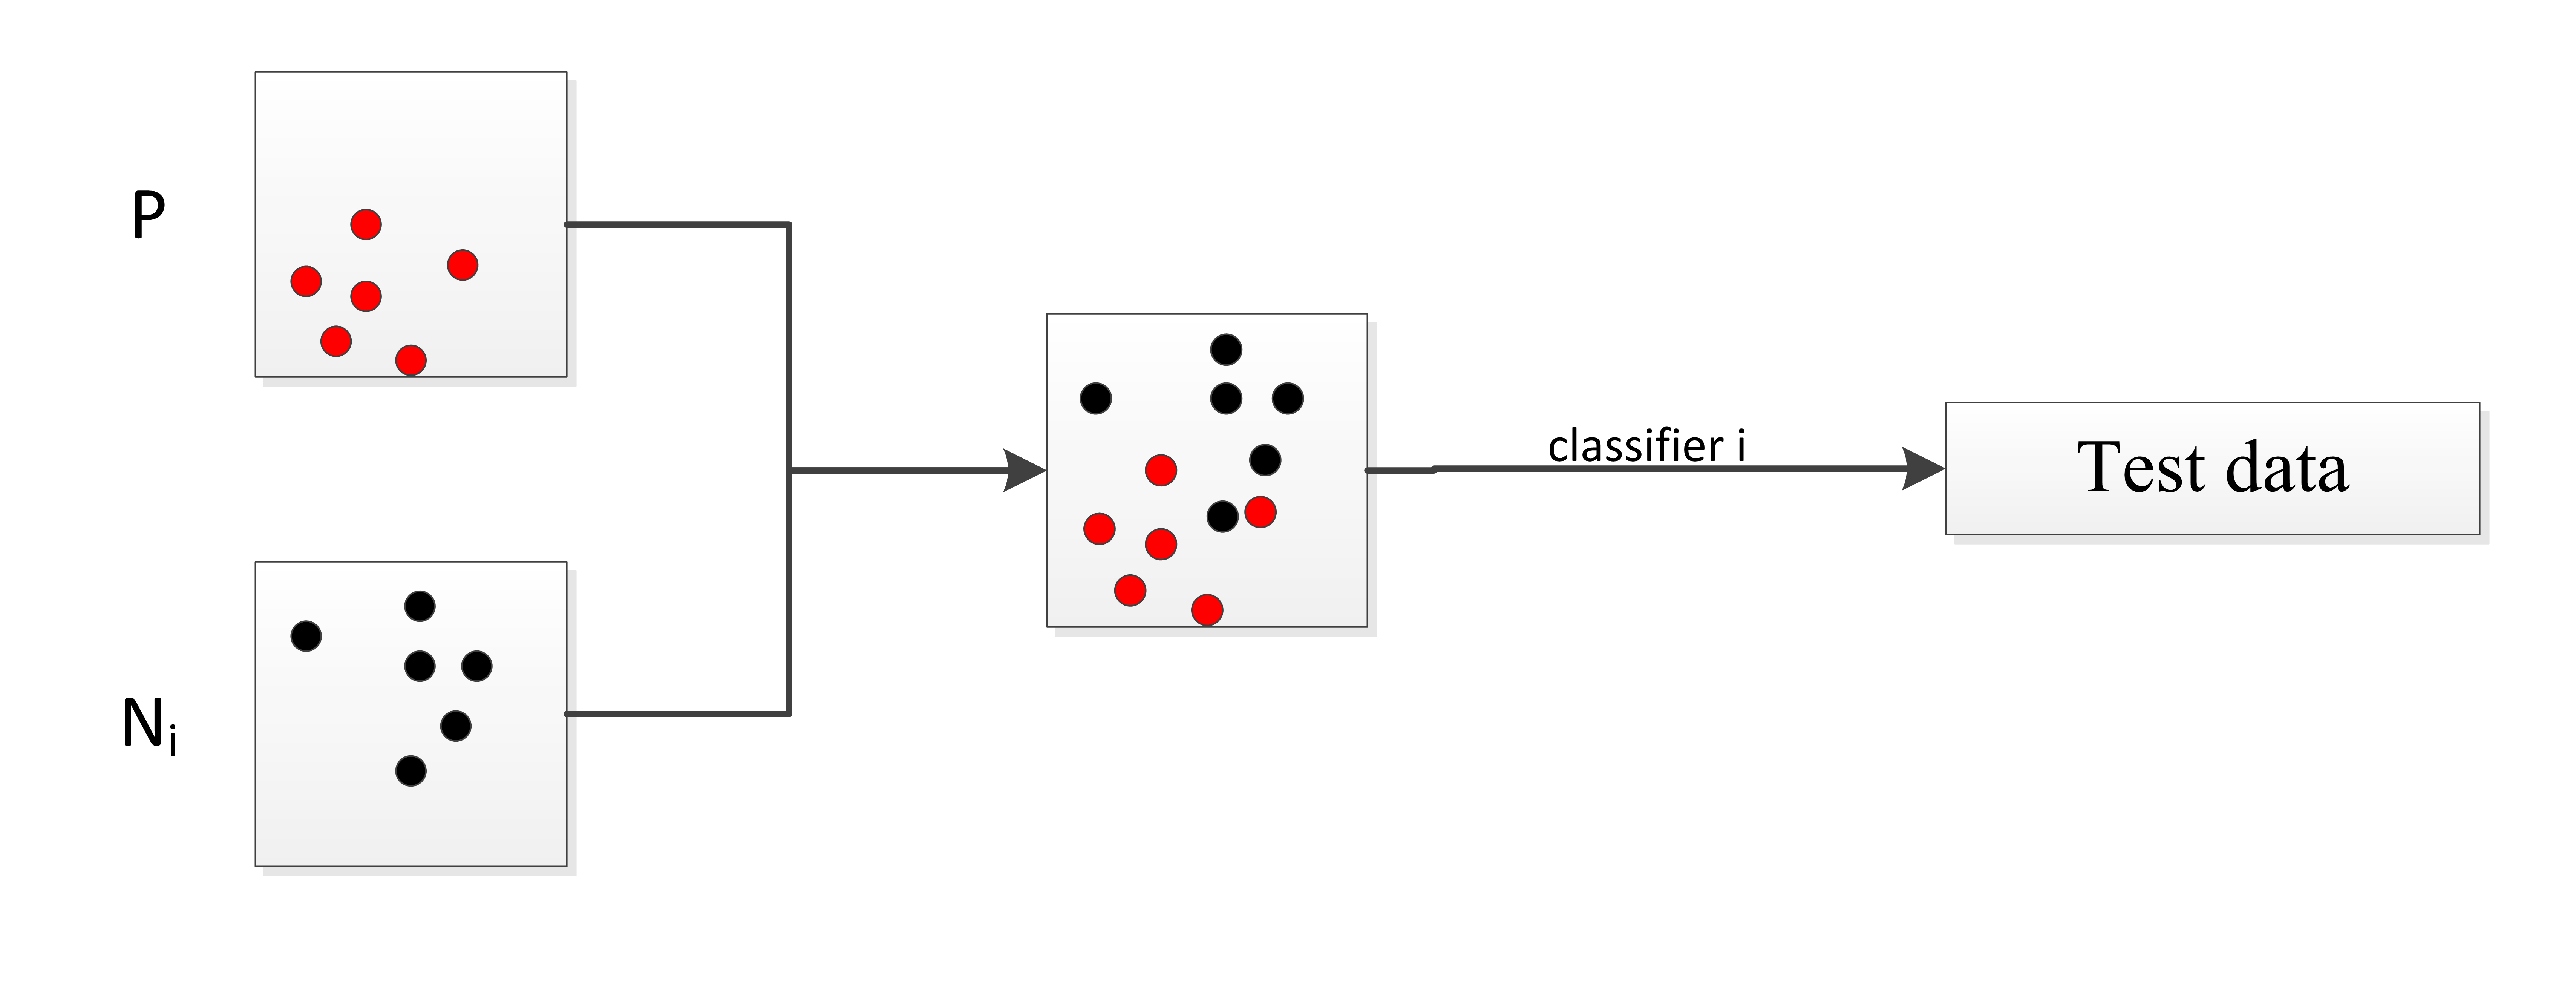
\includegraphics[width=0.55\linewidth]{method2}
%  \label{fig:b}
%\caption{method2}
  %\hspace{0.05in}  
\end{figure}
\end{frame}

\section{Experiment}

\begin{frame}{Datasets}
 
\begin{table}[hb]
    \centering
    \begin{tabular}{c|c|c}
        \hline 
        			&Sample		&IR\\
        \hline
        balance		&625		&11.8\\
        \hline
        car			&1728		&3.5\\
        \hline
        Colon		&62			&1.82\\
        \hline
        cmc			&1473		&3.4\\
        \hline
        Glioma		&50			&2.57\\
        \hline
        haberman	&306		&2.8\\
        \hline
        mf-morph	&2000		&9.0\\
        \hline
        mf-zernike	&2000		&9.0\\
        \hline
        vehicle		&846		&3.0\\
        \hline
        ZooScan		&2000		&15.25\\
        \hline 
        
	
    \end{tabular}
%    \caption{Datasets in the experiment.}
    \label{tab:datasets}
\end{table}


\end{frame}


\begin{frame}{Evaluation Criteria}

TN : true negatives\qquad \qquad
FP : false positives

TP : true positives\qquad \qquad 
FN : false negatives

$Precision: p = \frac{TP}{TP+FP}$

$Recal: r = \frac{TP}{TP+FN}$

$\textbf{acc} = \frac{TP+TN}{TP+FN+TN+FP}$

$\textbf{G-means} = \sqrt{TPR*TNR}$

$\textbf{F-measure} = \frac{1}{\frac{1}{2}(\frac{1}{p}+\frac{1}{r})} = \frac{2pr}{p+r}$

$Micro-F = \frac{1}{k}\sum^{k}_{i=1}F_{i}$

\textbf{AUC}: Area under the ROC curve

\end{frame}

\begin{frame}{SVM based on Gaussian radial basis kernel function}

	\begin{table}[hb]
    \centering
    \begin{tabular}{c|c}
        \hline 
        parameters of SVM	&value\\
        \hline 
        $\sigma$: the width of Gaussian radial basis kernel function		&5\\
        \hline 
        C: Penalty factor	&500\\
        \hline
    \end{tabular}
    %\caption{Parameters of SVM}
    \label{SVM}
\end{table}

\begin{table}[hb]
    \centering
    \begin{tabular}{c|c}
        \hline 
        parameters of ACOSampling	&value\\
        \hline 
        ant\_n		&50\\
        \hline 
        ITA		&50\\
        \hline
                ITP		&100\\
        \hline 
        dispose		&0.8\\
        \hline
        ph\_initial		&1\\
        \hline 
        $ph_{min}$		&0.5\\
        \hline
        $ph_{min}$		&0.5\\
        \hline
        $\alpha, \beta, \gamma$	&$\frac{1}{3}$\\
        \hline
    \end{tabular}
    %\caption{Parameters of AC}
    \label{aco}
\end{table}

\end{frame}

\section{Result}

\begin{frame}{Colon}

\begin{table}[!h]
  	\centering
      \scriptsize
	\begin{tabular}{c|c|c|c|c|c|c}
    \toprule[1.5pt]
    \hline
    			&ORI	&ROS	&RUS	&SMOTE	&BSO1	&BSO2	\\ 
	\hline
    Acc			&83.23	&84.19	&85.48	&85.48	&83.07	&84.03	\\
    \hline
     F-measure	&75.24	&76.78	&79.31	&79.37	&74.99	&76.91\\
	\hline
    G-mean		&80.23	&81.54	&84.17	&83.83	&80.01	&81.68	\\
	\hline
    AUC			&87.23	&87.76	&89.16	&89.13	&88.20	&88.61\\

        \midrule[1.2pt]

                &OSS	&ADA-SYN	&SBC	&ACOSampling	&Kernel-ADASYN	&KA-Ensemble\\
	\hline
    Acc			&85.65	&85.65		&83.23	&85.63		&85.63	&\textbf{86.03}\\
    \hline
     F-measure	&81.13	&79.76		&78.95	&81.13		&83.02	&\textbf{85.82}\\
	\hline
    G-mean		&85.76	&84.21	&84.25	&85.92	&\textbf{86.10}	&85.99	\\
	\hline
    AUC			&91.33	&88.82	&90.19	&94.18		&95.67	&\textbf{97.25}\\
    	\hline
\bottomrule[1.2pt]
    \end{tabular}
    %\caption{Results on full ZooScan}
    %\label{result4}    
   % \resizebox{\linewidth}{!}{\rule{1\linewidth}{3cm}}
\end{table}

\end{frame}

\begin{frame}{Glioma}

\begin{table}[!h]
  	\centering
      \scriptsize
	\begin{tabular}{c|c|c|c|c|c|c}
    \toprule[1.5pt]
    \hline
    			&ORI	&ROS	&RUS	&SMOTE	&BSO1	&BSO2	\\ 
	\hline
    Acc			&92.80	&94.00	&92.20	&93.60	&94.00	&93.40	\\
    \hline
     F-measure	&87.08	&89.35	&87.54	&88.56	&89.32	&88.80\\
	\hline
    G-mean		&90.94	&92.71	&93.16	&91.97	&92.47	&93.19	\\
	\hline
    AUC			&98.71	&98.93	&98.75	&98.87	&\textbf{99.15}	&98.73\\

        \midrule[1.2pt]

                &OSS	&ADA-SYN	&SBC	&ACOSampling	&Kernel-ADASYN	&KA-Ensemble\\
	\hline
    Acc			&68.21	&65.38	&67.18	&71.79	&72.00	&\textbf{75.21}	\\
    \hline
     F-measure	&62.50	&54.79	&60.43	&67.86	&67.84	&\textbf{69.10}\\
	\hline
    G-mean		&68.06	&62.67	&66.74	&72.32	&72.78	&\textbf{73.25}	\\
	\hline
    AUC			&73.53	&68.00	&73.22	&77.42	&\textbf{79.02}	&78.00\\
    	\hline
\bottomrule[1.2pt]
    \end{tabular}
    %\caption{Results on full ZooScan}
    %\label{result4}    
   % \resizebox{\linewidth}{!}{\rule{1\linewidth}{3cm}}
\end{table}

\end{frame}


\begin{frame}{ZooScan}

\begin{table}[!h]
  	\centering
      \scriptsize
	\begin{tabular}{c|c|c|c|c|c|c}
    \toprule[1.5pt]
    \hline
    			&ORI	&ROS	&RUS	&SMOTE	&BSO1	&BSO2	\\ 
	\hline
    Acc			&53.23	&64.19	&55.48	&55.48	&63.07	&64.03	\\
    \hline
     F-measure	&46.10	&43.30	&50.56	&45.58	&55.40	&49.39\\
	\hline
    G-mean		&53.46	&51.48	&56.89	&53.35	&52.93	&56.16	\\
	\hline
    AUC			&57.75	&57.36	&61.22	&57.92	&58.14	&59.78\\

        \midrule[1.2pt]

                &OSS	&ADA-SYN	&SBC	&ACOSampling	&Kernel-ADASYN	&KA-Ensemble\\
	\hline
    Acc			&58.16	&56.25		&55.48	&66.12			&66.66			&\textbf{71.26}	\\
    \hline
     F-measure	&52.83	&51.99		&50.56	&50.82			&52.64			&\textbf{57.33}\\
	\hline
    G-mean		&54.36	&58.37		&56.89	&53.89			&60.09			&\textbf{65.24}	\\
	\hline
    AUC			&57.35	&55.83		&51.22	&57.93			&62.37			&\textbf{68.80}\\
    	\hline
\bottomrule[1.2pt]
    \end{tabular}
    %\caption{Results on full ZooScan}
    \label{result4}    
   % \resizebox{\linewidth}{!}{\rule{1\linewidth}{3cm}}
\end{table}

\end{frame}


\begin{frame}
\centering\Huge\textsc{Q 1\& A}
\end{frame}

\end{document}
